% Étape Swin : les mêmes fenêtres, décalées d'une demi-fenêtre (FreeFlow)
% Compiler avec pdflatex (ou Overleaf).
\documentclass[border=10pt]{standalone}
\usepackage[T1]{fontenc}
\usepackage[utf8]{inputenc}
\usepackage[scaled]{helvet}
\renewcommand{\familydefault}{\sfdefault}
\usepackage{sansmath}
\sansmath
\usepackage{amsmath}
\usepackage{tikz}
\usetikzlibrary{arrows.meta}

% couleurs simples : couleur = fenêtre de Win (bleu, vert, jaune, rouge)
\definecolor{cA}{HTML}{9CC8F0}
\definecolor{cB}{HTML}{A8DCA0}
\definecolor{cC}{HTML}{FFE27A}
\definecolor{cD}{HTML}{F4A6A6}
\definecolor{orange}{HTML}{CCCCCC}
\definecolor{creme}{HTML}{F2F2F2}
\definecolor{bordeaux}{HTML}{222222}
\definecolor{grisclair}{HTML}{F2F2F2}

\tikzset{
  th/.style={font=\fontsize{14}{16}\selectfont\bfseries, text=black, inner sep=0pt},
  ts/.style={font=\fontsize{12}{14}\selectfont, text=black, inner sep=0pt},
  tm/.style={font=\fontsize{13}{15}\selectfont, text=black, inner sep=0pt},
  fl/.style={bordeaux, line width=1.5pt, -{Stealth[length=7pt]}},
}
\newcommand{\num}[1]{\tikz[baseline=(c.base)]\node[circle,draw=black,line width=0.7pt,inner sep=1pt,font=\fontsize{10}{10}\selectfont\bfseries](c){#1};}
% couleur de la fenêtre de Win (a, b) : damier de 4 teintes
\newcommand{\setwin}[2]{%
  \pgfmathtruncatemacro{\idx}{2*mod(#1,2)+mod(#2,2)}%
  \ifcase\idx \def\cc{cA}\or \def\cc{cB}\or \def\cc{cC}\or \def\cc{cD}\fi}
% grille 8 x 8 colorée par fenêtre de Win : \grille{x}{y}
\newcommand{\grille}[2]{%
  \foreach \a in {0,...,7} \foreach \b in {0,...,7} {
    \pgfmathtruncatemacro{\wa}{floor(\a/2)}
    \pgfmathtruncatemacro{\wb}{floor(\b/2)}
    \setwin{\wa}{\wb}
    \filldraw[fill=\cc, draw=white, line width=1pt] (#1+20*\b,#2+20*\a) rectangle ++(20,20);
  }}
% deux patchs voisins (ligne 3, colonnes 3 et 4)
\newcommand{\voisins}[2]{%
  \fill[bordeaux] (#1+70,#2+70) circle (4.5);
  \fill[bordeaux] (#1+90,#2+70) circle (4.5);}

\begin{document}
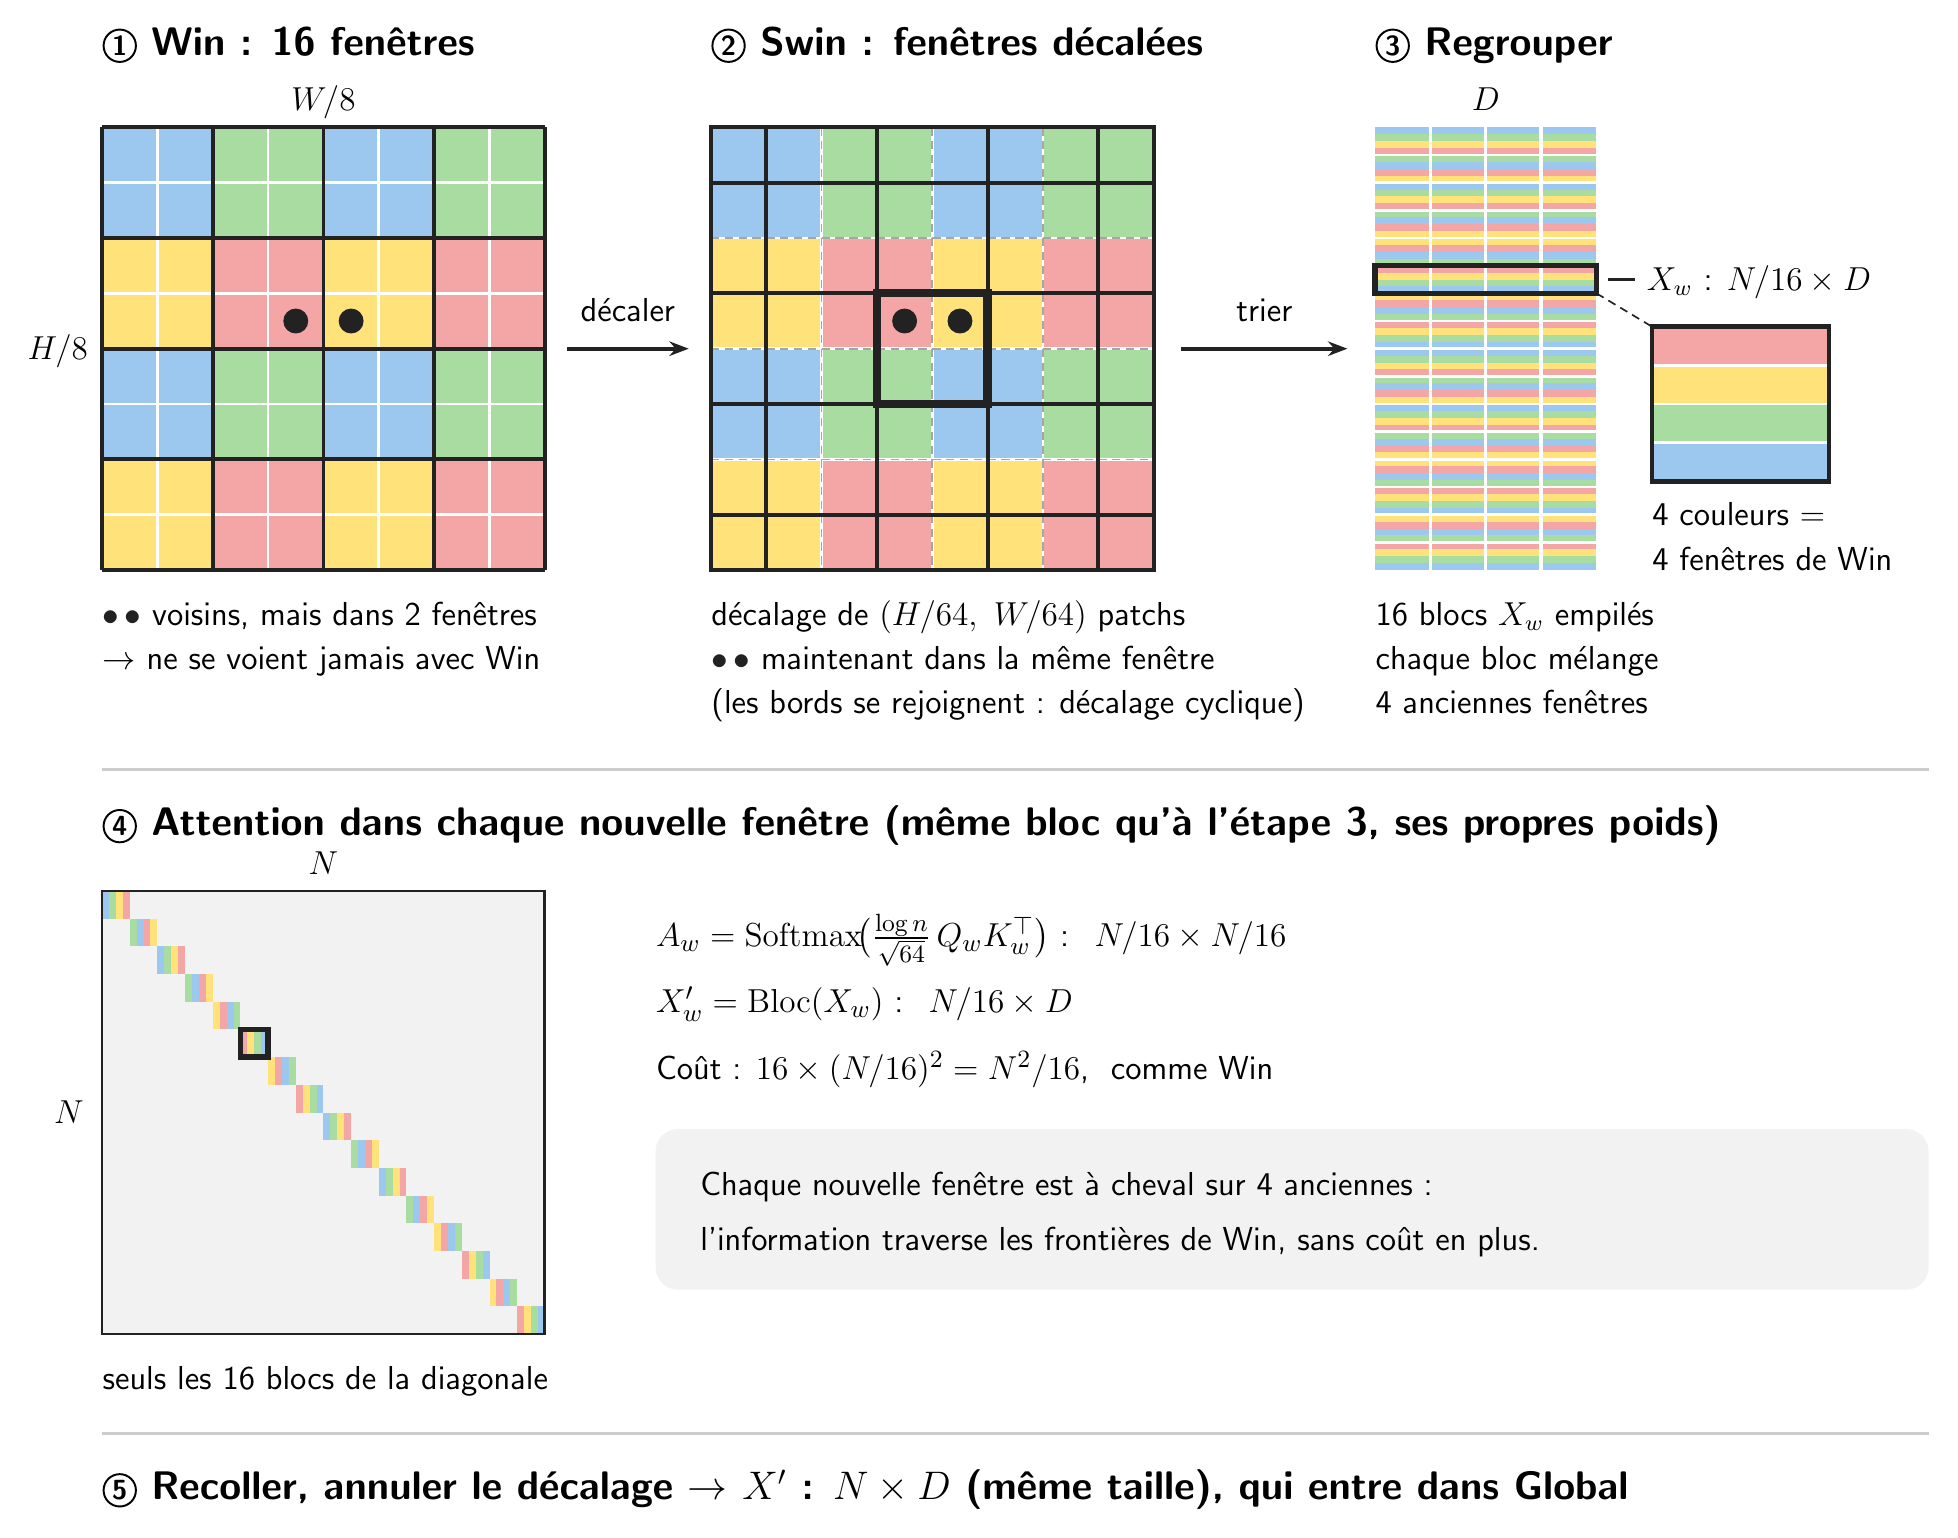
\begin{tikzpicture}[x=1pt, y=-1pt, line join=miter]

\node[th, anchor=base west] at (40,24)  {\num{1} Win : 16 fenêtres};
\node[th, anchor=base west] at (260,24) {\num{2} Swin : fenêtres décalées};
\node[th, anchor=base west] at (500,24) {\num{3} Regrouper};

% ---- 1. Win ----
\grille{40}{50}
\foreach \k in {0,...,4} {
  \draw[bordeaux, line width=1.4pt] (40+40*\k,50) -- ++(0,160);
  \draw[bordeaux, line width=1.4pt] (40,50+40*\k) -- ++(160,0);
}
\voisins{40}{50}
\node[ts, anchor=base] at (120,44) {$W/8$};
\node[ts, anchor=base] at (24,134) {$H/8$};
\node[ts, anchor=base west] at (40,230) {\textcolor{bordeaux}{$\bullet\,\bullet$} voisins, mais dans 2 fenêtres};
\node[ts, anchor=base west] at (40,246) {$\rightarrow$ ne se voient jamais avec Win};

\draw[fl] (208,130) -- (252,130);
\node[ts, anchor=base] at (230,120) {décaler};

% ---- 2. Swin : mêmes couleurs, nouvelles frontières ----
\grille{260}{50}
\foreach \k in {0,...,4} {
  \draw[black!35, line width=0.6pt, dash pattern=on 3pt off 2pt] (260+40*\k,50) -- ++(0,160);
  \draw[black!35, line width=0.6pt, dash pattern=on 3pt off 2pt] (260,50+40*\k) -- ++(160,0);
}
\foreach \k in {0,...,3} {
  \draw[bordeaux, line width=1.4pt] (280+40*\k,50) -- ++(0,160);
  \draw[bordeaux, line width=1.4pt] (260,70+40*\k) -- ++(160,0);
}
\draw[bordeaux, line width=1.4pt] (260,50) rectangle (420,210);
\draw[bordeaux, line width=3pt] (320,110) rectangle (360,150);
\voisins{260}{50}
\node[ts, anchor=base west] at (260,230) {décalage de $(H/64,\ W/64)$ patchs};
\node[ts, anchor=base west] at (260,246) {\textcolor{bordeaux}{$\bullet\,\bullet$} maintenant dans la même fenêtre};
\node[ts, anchor=base west] at (260,262) {(les bords se rejoignent : décalage cyclique)};

\draw[fl] (430,130) -- (490,130);
\node[ts, anchor=base] at (460,120) {trier};

% ---- 3. X~ trié par nouvelle fenêtre : chaque bloc mélange 4 couleurs ----
\foreach \A in {0,...,3} \foreach \B in {0,...,3} \foreach \m in {0,...,3} {
  \pgfmathtruncatemacro{\r}{mod(2*\A+1+floor(\m/2),8)}
  \pgfmathtruncatemacro{\c}{mod(2*\B+1+mod(\m,2),8)}
  \pgfmathtruncatemacro{\wa}{floor(\r/2)}
  \pgfmathtruncatemacro{\wb}{floor(\c/2)}
  \setwin{\wa}{\wb}
  \fill[\cc] (500,50+40*\A+10*\B+2.5*\m) rectangle ++(80,2.5);
}
\foreach \x in {520,540,560} \draw[white, line width=1.2pt] (\x,50) -- (\x,210);
\foreach \k in {1,...,15} \draw[white, line width=1pt] (500,50+10*\k) -- (580,50+10*\k);
\draw[bordeaux, line width=2pt] (500,100) rectangle (580,110);
\node[ts, anchor=base] at (540,44) {$D$};
\draw[bordeaux, line width=0.8pt] (584,105) -- (594,105);
\node[ts, anchor=base west] at (598,109) {$X_w$ : $N/16 \times D$};
% zoom sur le bloc encadré : ses 4 lignes viennent de 4 fenêtres de Win
\foreach \m in {0,...,3} {
  \pgfmathtruncatemacro{\r}{mod(3+floor(\m/2),8)}
  \pgfmathtruncatemacro{\c}{mod(3+mod(\m,2),8)}
  \pgfmathtruncatemacro{\wa}{floor(\r/2)}
  \pgfmathtruncatemacro{\wb}{floor(\c/2)}
  \setwin{\wa}{\wb}
  \filldraw[fill=\cc, draw=white, line width=1pt] (600,122+14*\m) rectangle ++(64,14);
}
\draw[bordeaux, line width=1.5pt] (600,122) rectangle (664,178);
\draw[bordeaux, line width=0.6pt, dash pattern=on 3pt off 2pt] (580,110) -- (600,122);
\node[ts, anchor=base west] at (600,194) {4 couleurs =};
\node[ts, anchor=base west] at (600,210) {4 fenêtres de Win};
\node[ts, anchor=base west] at (500,230) {16 blocs $X_w$ empilés};
\node[ts, anchor=base west] at (500,246) {chaque bloc mélange};
\node[ts, anchor=base west] at (500,262) {4 anciennes fenêtres};

% =============== LIGNE 2 ===============
\draw[orange, line width=1pt] (40,282) -- (700,282);
\node[th, anchor=base west] at (40,306) {\num{4} Attention dans chaque nouvelle fenêtre (même bloc qu'à l'étape 3, ses propres poids)};

\fill[grisclair] (40,326) rectangle (200,486);
\foreach \k in {0,...,15} {
  \pgfmathtruncatemacro{\A}{floor(\k/4)}
  \pgfmathtruncatemacro{\B}{mod(\k,4)}
  \foreach \m in {0,...,3} {
    \pgfmathtruncatemacro{\r}{mod(2*\A+1+floor(\m/2),8)}
    \pgfmathtruncatemacro{\c}{mod(2*\B+1+mod(\m,2),8)}
    \pgfmathtruncatemacro{\wa}{floor(\r/2)}
    \pgfmathtruncatemacro{\wb}{floor(\c/2)}
    \setwin{\wa}{\wb}
    \fill[\cc] (40+10*\k+2.5*\m,326+10*\k) rectangle ++(2.5,10);
  }
}
\draw[bordeaux, line width=1pt] (40,326) rectangle (200,486);
\draw[bordeaux, line width=2pt] (90,376) rectangle (100,386);
\node[ts, anchor=base] at (120,320) {$N$};
\node[ts, anchor=base] at (28,410) {$N$};
\node[ts, anchor=base west] at (40,506) {seuls les 16 blocs de la diagonale};

\node[tm, anchor=base west] at (240,346) {$A_w = \mathrm{Softmax}\!\big(\tfrac{\log n}{\sqrt{64}}\, Q_w K_w^{\top}\big)$ : \ $N/16 \times N/16$};
\node[tm, anchor=base west] at (240,370) {$X'_w = \mathrm{Bloc}(X_w)$ : \ $N/16 \times D$};
\node[tm, anchor=base west] at (240,394) {Coût : $16 \times (N/16)^2 = N^2/16$, \ comme Win};

\fill[creme, rounded corners=8pt] (240,412) rectangle (700,470);
\node[tm, anchor=base west] at (256,436) {Chaque nouvelle fenêtre est à cheval sur 4 anciennes :};
\node[tm, anchor=base west] at (256,456) {l'information traverse les frontières de Win, sans coût en plus.};

% =============== LIGNE 3 ===============
\draw[orange, line width=1pt] (40,522) -- (700,522);
\node[th, anchor=base west] at (40,546) {\num{5} Recoller, annuler le décalage $\rightarrow$ $X'$ : $N \times D$ (même taille), qui entre dans Global};

\end{tikzpicture}
\end{document}
